\documentclass[]{book}
\usepackage{lmodern}
\usepackage{amssymb,amsmath}
\usepackage{ifxetex,ifluatex}
\usepackage{fixltx2e} % provides \textsubscript
\ifnum 0\ifxetex 1\fi\ifluatex 1\fi=0 % if pdftex
  \usepackage[T1]{fontenc}
  \usepackage[utf8]{inputenc}
\else % if luatex or xelatex
  \ifxetex
    \usepackage{mathspec}
  \else
    \usepackage{fontspec}
  \fi
  \defaultfontfeatures{Ligatures=TeX,Scale=MatchLowercase}
\fi
% use upquote if available, for straight quotes in verbatim environments
\IfFileExists{upquote.sty}{\usepackage{upquote}}{}
% use microtype if available
\IfFileExists{microtype.sty}{%
\usepackage{microtype}
\UseMicrotypeSet[protrusion]{basicmath} % disable protrusion for tt fonts
}{}
\usepackage[margin=1in]{geometry}
\usepackage{hyperref}
\hypersetup{unicode=true,
            pdftitle={Traitement des données PMSI avec R},
            pdfauthor={Guillaume Pressiat},
            pdfborder={0 0 0},
            breaklinks=true}
\urlstyle{same}  % don't use monospace font for urls
\usepackage{natbib}
\bibliographystyle{plainnat}
\usepackage{color}
\usepackage{fancyvrb}
\newcommand{\VerbBar}{|}
\newcommand{\VERB}{\Verb[commandchars=\\\{\}]}
\DefineVerbatimEnvironment{Highlighting}{Verbatim}{commandchars=\\\{\}}
% Add ',fontsize=\small' for more characters per line
\usepackage{framed}
\definecolor{shadecolor}{RGB}{248,248,248}
\newenvironment{Shaded}{\begin{snugshade}}{\end{snugshade}}
\newcommand{\KeywordTok}[1]{\textcolor[rgb]{0.13,0.29,0.53}{\textbf{{#1}}}}
\newcommand{\DataTypeTok}[1]{\textcolor[rgb]{0.13,0.29,0.53}{{#1}}}
\newcommand{\DecValTok}[1]{\textcolor[rgb]{0.00,0.00,0.81}{{#1}}}
\newcommand{\BaseNTok}[1]{\textcolor[rgb]{0.00,0.00,0.81}{{#1}}}
\newcommand{\FloatTok}[1]{\textcolor[rgb]{0.00,0.00,0.81}{{#1}}}
\newcommand{\ConstantTok}[1]{\textcolor[rgb]{0.00,0.00,0.00}{{#1}}}
\newcommand{\CharTok}[1]{\textcolor[rgb]{0.31,0.60,0.02}{{#1}}}
\newcommand{\SpecialCharTok}[1]{\textcolor[rgb]{0.00,0.00,0.00}{{#1}}}
\newcommand{\StringTok}[1]{\textcolor[rgb]{0.31,0.60,0.02}{{#1}}}
\newcommand{\VerbatimStringTok}[1]{\textcolor[rgb]{0.31,0.60,0.02}{{#1}}}
\newcommand{\SpecialStringTok}[1]{\textcolor[rgb]{0.31,0.60,0.02}{{#1}}}
\newcommand{\ImportTok}[1]{{#1}}
\newcommand{\CommentTok}[1]{\textcolor[rgb]{0.56,0.35,0.01}{\textit{{#1}}}}
\newcommand{\DocumentationTok}[1]{\textcolor[rgb]{0.56,0.35,0.01}{\textbf{\textit{{#1}}}}}
\newcommand{\AnnotationTok}[1]{\textcolor[rgb]{0.56,0.35,0.01}{\textbf{\textit{{#1}}}}}
\newcommand{\CommentVarTok}[1]{\textcolor[rgb]{0.56,0.35,0.01}{\textbf{\textit{{#1}}}}}
\newcommand{\OtherTok}[1]{\textcolor[rgb]{0.56,0.35,0.01}{{#1}}}
\newcommand{\FunctionTok}[1]{\textcolor[rgb]{0.00,0.00,0.00}{{#1}}}
\newcommand{\VariableTok}[1]{\textcolor[rgb]{0.00,0.00,0.00}{{#1}}}
\newcommand{\ControlFlowTok}[1]{\textcolor[rgb]{0.13,0.29,0.53}{\textbf{{#1}}}}
\newcommand{\OperatorTok}[1]{\textcolor[rgb]{0.81,0.36,0.00}{\textbf{{#1}}}}
\newcommand{\BuiltInTok}[1]{{#1}}
\newcommand{\ExtensionTok}[1]{{#1}}
\newcommand{\PreprocessorTok}[1]{\textcolor[rgb]{0.56,0.35,0.01}{\textit{{#1}}}}
\newcommand{\AttributeTok}[1]{\textcolor[rgb]{0.77,0.63,0.00}{{#1}}}
\newcommand{\RegionMarkerTok}[1]{{#1}}
\newcommand{\InformationTok}[1]{\textcolor[rgb]{0.56,0.35,0.01}{\textbf{\textit{{#1}}}}}
\newcommand{\WarningTok}[1]{\textcolor[rgb]{0.56,0.35,0.01}{\textbf{\textit{{#1}}}}}
\newcommand{\AlertTok}[1]{\textcolor[rgb]{0.94,0.16,0.16}{{#1}}}
\newcommand{\ErrorTok}[1]{\textcolor[rgb]{0.64,0.00,0.00}{\textbf{{#1}}}}
\newcommand{\NormalTok}[1]{{#1}}
\usepackage{longtable,booktabs}
\usepackage{graphicx,grffile}
\makeatletter
\def\maxwidth{\ifdim\Gin@nat@width>\linewidth\linewidth\else\Gin@nat@width\fi}
\def\maxheight{\ifdim\Gin@nat@height>\textheight\textheight\else\Gin@nat@height\fi}
\makeatother
% Scale images if necessary, so that they will not overflow the page
% margins by default, and it is still possible to overwrite the defaults
% using explicit options in \includegraphics[width, height, ...]{}
\setkeys{Gin}{width=\maxwidth,height=\maxheight,keepaspectratio}
\IfFileExists{parskip.sty}{%
\usepackage{parskip}
}{% else
\setlength{\parindent}{0pt}
\setlength{\parskip}{6pt plus 2pt minus 1pt}
}
\setlength{\emergencystretch}{3em}  % prevent overfull lines
\providecommand{\tightlist}{%
  \setlength{\itemsep}{0pt}\setlength{\parskip}{0pt}}
\setcounter{secnumdepth}{5}
% Redefines (sub)paragraphs to behave more like sections
\ifx\paragraph\undefined\else
\let\oldparagraph\paragraph
\renewcommand{\paragraph}[1]{\oldparagraph{#1}\mbox{}}
\fi
\ifx\subparagraph\undefined\else
\let\oldsubparagraph\subparagraph
\renewcommand{\subparagraph}[1]{\oldsubparagraph{#1}\mbox{}}
\fi

%%% Use protect on footnotes to avoid problems with footnotes in titles
\let\rmarkdownfootnote\footnote%
\def\footnote{\protect\rmarkdownfootnote}

%%% Change title format to be more compact
\usepackage{titling}

% Create subtitle command for use in maketitle
\newcommand{\subtitle}[1]{
  \posttitle{
    \begin{center}\large#1\end{center}
    }
}

\setlength{\droptitle}{-2em}
  \title{Traitement des données PMSI avec R}
  \pretitle{\vspace{\droptitle}\centering\huge}
  \posttitle{\par}
  \author{Guillaume Pressiat}
  \preauthor{\centering\large\emph}
  \postauthor{\par}
  \predate{\centering\large\emph}
  \postdate{\par}
  \date{2017-02-10}

\usepackage{booktabs}
\usepackage{amsthm}
\makeatletter
\def\thm@space@setup{%
  \thm@preskip=8pt plus 2pt minus 4pt
  \thm@postskip=\thm@preskip
}
\makeatother

\begin{document}
\maketitle

{
\setcounter{tocdepth}{1}
\tableofcontents
}
\chapter{Introduction}\label{introduction}

Ce livre numérique présente des exemples de traitements de données PMSI
avec R. L'objectif est de concentrer ici :

\begin{itemize}
\tightlist
\item
  une documentation permettant de débuter avec l'import de données via
  le package \emph{pmeasyr}
\end{itemize}

et des exemples d'analyses PMSI :

\begin{itemize}
\tightlist
\item
  étude de la durée moyenne de séjour
\item
  requêtes sur les diagnostics et les actes
\item
  analyse des files actives pour une pathologie
\item
  chainage PMSI de patients
\item
  reporting de l'activité
\item
  visualisation graphiques, cartographies
\end{itemize}

\chapter{Contexte et motivations}\label{contexte}

Les données du Programme de Médicalisation des Systèmes d'Informations
(PMSI) sont souvent traitées via des logiciels spécifiques au PMSI (ou
des outils statistiques / bases de données du marché) ne permettant pas
de réaliser des traitements statistiques et des infographies
satisfaisantes. Les départements d'information médicale sont donc
souvent amenés à retraiter ces données avec R.

L'évolution récente de R intègre la manipulation de bases de données de
taille importante. Le package \emph{pmeasyr} s'inscrit dans cette veine
et permet de réaliser de façon autonome l'ensemble des traitements (de
l'import des données à leur analyse) avec R.

\section{Avantages de R}\label{avantages-de-r}

\subsection{Un flux de travail unique}\label{un-flux-de-travail-unique}

En travaillant uniquement avec R, on peut mettre en place un flux de
travail épuré : un seul projet, un seul programme, un seul logiciel. La
traçabilité, la reproductibilité et la mise à jour des opérations sont
ainsi facilitées.

Le travail avec de multiples logiciels oblige à l'export / import de
fichiers entre les différents logiciels, et chaque modification du début
du flux de travail génère des fichiers exportés v1, v2, \ldots{}

Avec un flux complet dans R, toute nouvelle modification est intégrée au
processus de travail global. La localisation de toutes les étapes d'une
analyse en un seul point évite les erreurs et la confusion lorsque l'on
reprend l'analyse ultérieurement.

\subsection{R et le PMSI}\label{r-et-le-pmsi}

L'utilisation de R confère aux données du PMSI la liberté proposée par
le logiciel :

\begin{itemize}
\tightlist
\item
  les requêtes sur les diagnostics et les actes peuvent s'écrire de
  multiples façons et c'est l'utilisateur qui crée ses propres
  programmes
\item
  les données sont dans R : prêtes pour des modèles linéaires,
  logistiques, des classifications\ldots{}
\item
  la confrontation des données in* (reflet du codage des établissements)
  aux données out* (reflet de la valorisation accordée à
  l'établissement) est facilitée par l'import du fichier tra, cela peut
  permettre aux équipes DIM d'améliorer leur recueil\\
\item
  le reporting de l'activité en excel, pdf, word, html, ou en créant des
  applications (shiny)
\item
  l'utilisation des graphiques pour représenter des volumes d'activités
  et des cartographies interactives pour visualiser la localisation
  d'activités, de patientèles, et les flux de patients
\item
  le partage de projets RStudio, qui facilite et encourage les travaux
  en équipe.
\end{itemize}

**NB: Données In / Out : données en entrée / sortie des logiciels de
l'ATIH*

\subsection{Des outils performants}\label{des-outils-performants}

L'engouement autour de R est lié au développement de packages intuitifs
et performants : \emph{readr}, \emph{dplyr}, \emph{tidyr},
\emph{magrittr}, pour n'en citer que quelques-uns. \emph{pmeasyr}
s'appuie sur ces packages pour proposer des imports de données rapides
sur des fichiers de taille importante (l'entité juridique de l'AP-HP est
prise en charge sans problème avec un ordinateur récent).

Dans le cas de \emph{pmeasyr}, l'import de 100 000 rsa (partie fixe,
parsing des passages unités médicales, des diagnostics associés et des
actes) nécessite en moyenne 5 secondes avec un processeur i7 -- 16Go de
ram.

En dernier ressort, R travaillant en mémoire vive, les exécutions de
requêtes sont très rapides.

\section{Contenu du package}\label{contenu-du-package}

Le package contient des fonctions pour la gestion des archives PMSI en
entrée / sortie des logiciels de l'ATIH : dézippage, suppression des
archives, et des fonctions pour l'import des fichiers des champs PMSI
MCO, SSR, HAD, PSY et RSF.

Il est utilisé depuis un an à l'AP-HP pour des analyses d'activité et la
description des prises en charge.

\section{Installation du package}\label{installation-du-package}

\textbf{Depuis github avec devtools}

\begin{Shaded}
\begin{Highlighting}[]
\NormalTok{devtools::}\KeywordTok{install_github}\NormalTok{(}\StringTok{'IM-APHP/pmeasyr'}\NormalTok{)}
\end{Highlighting}
\end{Shaded}

Cette commande lance l'installation du package et de ses dépendances.

\chapter{Les archives PMSI}\label{archives}

Cette partie aborde le point de départ des études PMSI : les archives
PMSI. Ces archives sont les fichiers en entrées / sorties des logiciels
de l'ATIH.

Les manuels techniques de ces logiciels,relatifs aux champs MCO, SSR,
HAD, PSY et RSF, respectivement
\href{http://atih.sante.fr/plateformes-de-transmission-et-logiciels/logiciels-espace-de-telechargement\#G}{Genrsa},
\href{http://atih.sante.fr/plateformes-de-transmission-et-logiciels/logiciels-espace-de-telechargement\#G}{Genrha},
\href{http://atih.sante.fr/plateformes-de-transmission-et-logiciels/logiciels-espace-de-telechargement\#P}{Paprica},
\href{http://atih.sante.fr/plateformes-de-transmission-et-logiciels/logiciels-espace-de-telechargement\#P}{Pivoine}
et
\href{http://atih.sante.fr/plateformes-de-transmission-et-logiciels/logiciels-espace-de-telechargement\#P}{Preface}
sont disponibnles dans
l'\href{http://atih.sante.fr/plateformes-de-transmission-et-logiciels/logiciels-espace-de-telechargement}{espace
de telechargement} sur le site de l'ATIH.

\subsection{Gestion des archives dans des
répertoires}\label{gestion-des-archives-dans-des-repertoires}

Le package \emph{pmeasyr} prend en charge les données des quatre champs
PMSI MCO, SSR, HAD, PSY ainsi que les RSF.

Placer les archives dans un répertoire, par exemple ici dans
\texttt{\textasciitilde{}/Documents/data/mco} :

\begin{figure}[htbp]
\centering
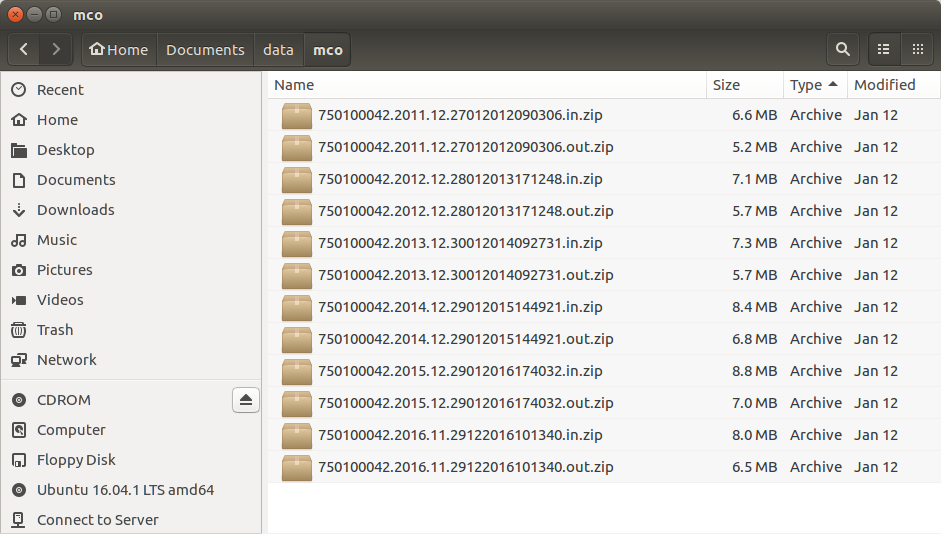
\includegraphics{images/archives_mco.png}
\caption{Archives MCO}
\end{figure}

Vous noterez que pour chaque champ PMSI il est conseillé d'utiliser un
répertoire indépendant, ceci est nécessaire dans la mesure où le nom des
archives PMSI ne contient pas l'information champ MCO, RSF, etc., il
faut organiser l'archivage champ par champ, dans des répertoires
différents.

\begin{figure}[htbp]
\centering
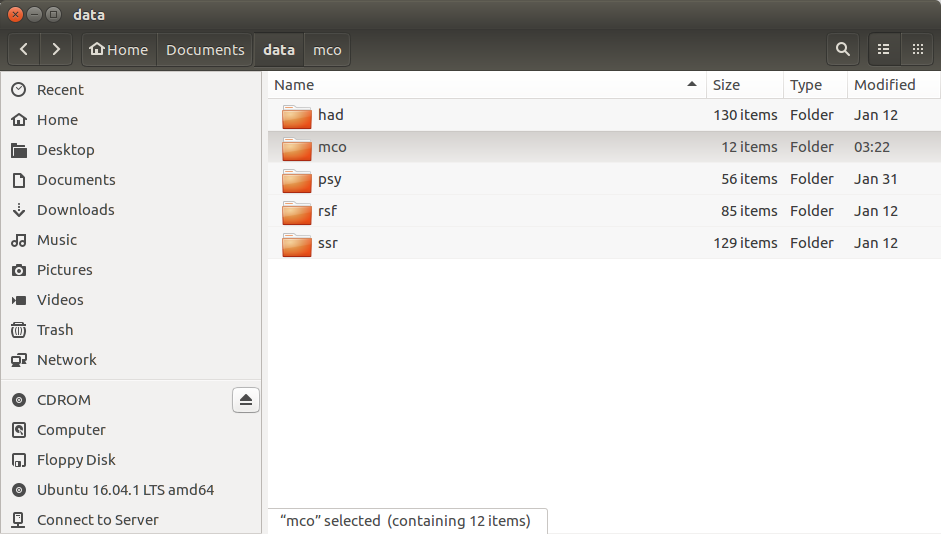
\includegraphics{images/champ_par_champ.png}
\caption{Un répertoire par champ PMSI}
\end{figure}

\begin{Shaded}
\begin{Highlighting}[]
\CommentTok{# Créer l'arborescence à partir de R}
\NormalTok{champs =}\StringTok{ }\KeywordTok{c}\NormalTok{(}\StringTok{'mco'}\NormalTok{, }\StringTok{'ssr'}\NormalTok{, }\StringTok{'had'}\NormalTok{, }\StringTok{'psy'}\NormalTok{, }\StringTok{'rsf'}\NormalTok{)}
\NormalTok{emplacement <-}\StringTok{ "~/Documents/data"}
\KeywordTok{sapply}\NormalTok{(champs, function(x)\{}\KeywordTok{dir.create}\NormalTok{(}\KeywordTok{file.path}\NormalTok{(emplacement, x))\})}
\end{Highlighting}
\end{Shaded}

\subsection{Informations sur les
archives}\label{informations-sur-les-archives}

La fonction \texttt{astat} permet d'éditer des statistiques sommaires
sur les fichiers contenus dans une archive.

\begin{longtable}[]{@{}ll@{}}
\toprule
Nom & Fonction\tabularnewline
\midrule
\endhead
\href{https://github.com/IM-APHP/pmeasyr/tree/master/Rd_md/astat.Rmd}{astat}
& \textasciitilde{} *.zip - Liste et volume des fichiers d'une archive
PMSI\tabularnewline
\bottomrule
\end{longtable}

\begin{Shaded}
\begin{Highlighting}[]
\CommentTok{# Informations sur les fichiers : Date de creation, Taille}
\NormalTok{pmeasyr::}\KeywordTok{astat}\NormalTok{(}\DataTypeTok{path =} \StringTok{'~/Documents/data/mco/'}\NormalTok{, }
               \DataTypeTok{file =} \StringTok{'750100042.2015.12.29012016174032.out.zip'}\NormalTok{, }
               \DataTypeTok{view =} \NormalTok{F)}
\end{Highlighting}
\end{Shaded}

\subsection{Dézippage}\label{dezippage}

Cette partie du package facilite la manipulation des archives PMSI,
fichiers de type :

\begin{itemize}
\tightlist
\item
  \texttt{finess.annee.mois.date\_et\_heure\_de\_creation.in.zip}
\item
  \texttt{finess.annee.mois.date\_et\_heure\_de\_creation.out.zip}
\end{itemize}

Les fonctions permettent de dezipper les fichiers depuis \texttt{R} en
ligne de commande, sans intervention manuelle de l'utilisateur.
L'avantage est d'obtenir un processus ne relevant pas d'interventions
externes au logiciel \texttt{R} (pour pouvoir garder trace des etapes,
et faciliter la reproduction, tout est inscrit dans un programme, dans
un flux de processus). Une fois que les traitements et analyses sur les
fichiers sont faits, il est possible d'effacer les archives egalement en
ligne de commande.

Le nom des fonctions dont l'objectif est de manipuler les
\textbf{a}rchives commence par \textbf{a}.

\begin{longtable}[]{@{}ll@{}}
\toprule
\begin{minipage}[b]{0.10\columnwidth}\raggedright\strut
Nom\strut
\end{minipage} & \begin{minipage}[b]{0.84\columnwidth}\raggedright\strut
Fonction\strut
\end{minipage}\tabularnewline
\midrule
\endhead
\begin{minipage}[t]{0.10\columnwidth}\raggedright\strut
\href{https://github.com/IM-APHP/pmeasyr/tree/master/Rd_md/adezip.Rmd}{adezip}\strut
\end{minipage} & \begin{minipage}[t]{0.84\columnwidth}\raggedright\strut
\textasciitilde{} *.zip - Dezippe des fichiers de larchive PMSI\strut
\end{minipage}\tabularnewline
\begin{minipage}[t]{0.10\columnwidth}\raggedright\strut
\href{https://github.com/IM-APHP/pmeasyr/tree/master/Rd_md/adezip2.Rmd}{adezip2}\strut
\end{minipage} & \begin{minipage}[t]{0.84\columnwidth}\raggedright\strut
\textasciitilde{} *.zip - Dezippe des fichiers de l'archive PMSI, avec
en parametre le nom de l'archive\strut
\end{minipage}\tabularnewline
\bottomrule
\end{longtable}

\begin{Shaded}
\begin{Highlighting}[]
\CommentTok{# Dezippage uniquement des fichiers rsa, ano et tra du out 2015}
\CommentTok{# Ex: 750100042.2015.12.20160130.153012.out.zip}
\NormalTok{pmeasyr::}\KeywordTok{adezip}\NormalTok{(}\DataTypeTok{finess =} \DecValTok{750100042}\NormalTok{, }
                \DataTypeTok{annee =} \DecValTok{2015}\NormalTok{, }
                \DataTypeTok{mois =} \DecValTok{12}\NormalTok{, }
                \DataTypeTok{path =} \StringTok{'~/Documents/data/mco'}\NormalTok{, }
                \DataTypeTok{liste =} \KeywordTok{c}\NormalTok{(}\StringTok{"rsa"}\NormalTok{, }\StringTok{"ano"}\NormalTok{, }\StringTok{"tra"}\NormalTok{), }
                \DataTypeTok{type =} \StringTok{"out"}\NormalTok{)}
\end{Highlighting}
\end{Shaded}

\begin{figure}[htbp]
\centering
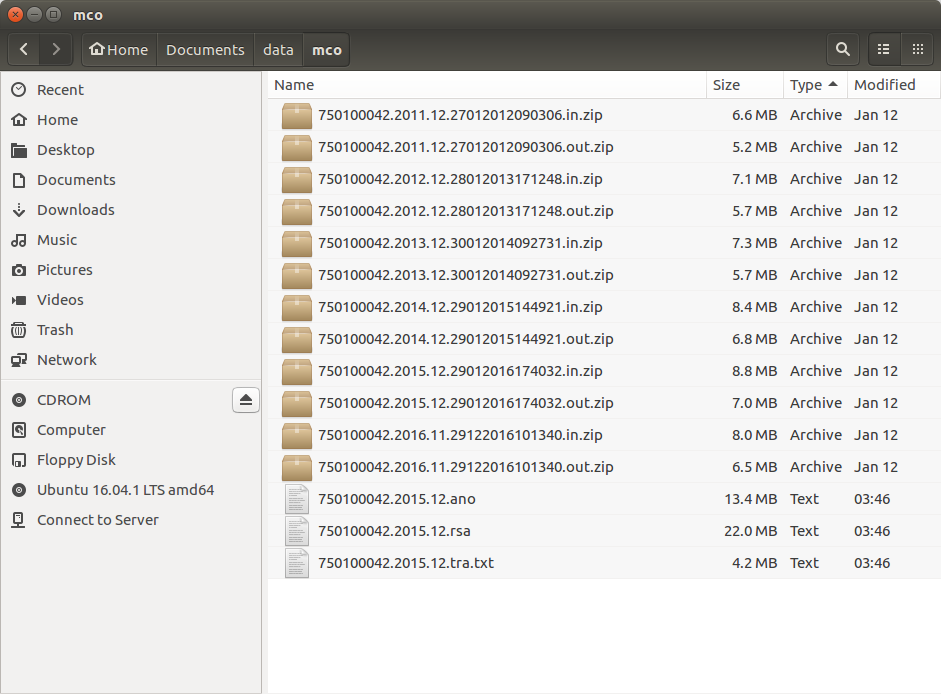
\includegraphics{images/archives_dezip.png}
\caption{Après éxécution de \texttt{adezip()} sur des fichiers du
\emph{out}}
\end{figure}

\begin{Shaded}
\begin{Highlighting}[]
\CommentTok{# Dezippage uniquement des fichiers rss, dmi et med du in 2014}
\CommentTok{# Ex: 750100042.2015.12.20160130.153012.out.zip}
\NormalTok{pmeasyr::}\KeywordTok{adezip}\NormalTok{(}\DataTypeTok{finess =} \DecValTok{750100042}\NormalTok{, }
                \DataTypeTok{annee =} \DecValTok{2015}\NormalTok{, }
                \DataTypeTok{mois =} \DecValTok{12}\NormalTok{, }
                \DataTypeTok{path =} \StringTok{'~/Documents/data/mco'}\NormalTok{, }
                \DataTypeTok{liste =} \KeywordTok{c}\NormalTok{(}\StringTok{"rss"}\NormalTok{, }\StringTok{"dmi"}\NormalTok{, }\StringTok{"med"}\NormalTok{), }
                \DataTypeTok{type =} \StringTok{"in"}\NormalTok{)}
\end{Highlighting}
\end{Shaded}

\begin{figure}[htbp]
\centering
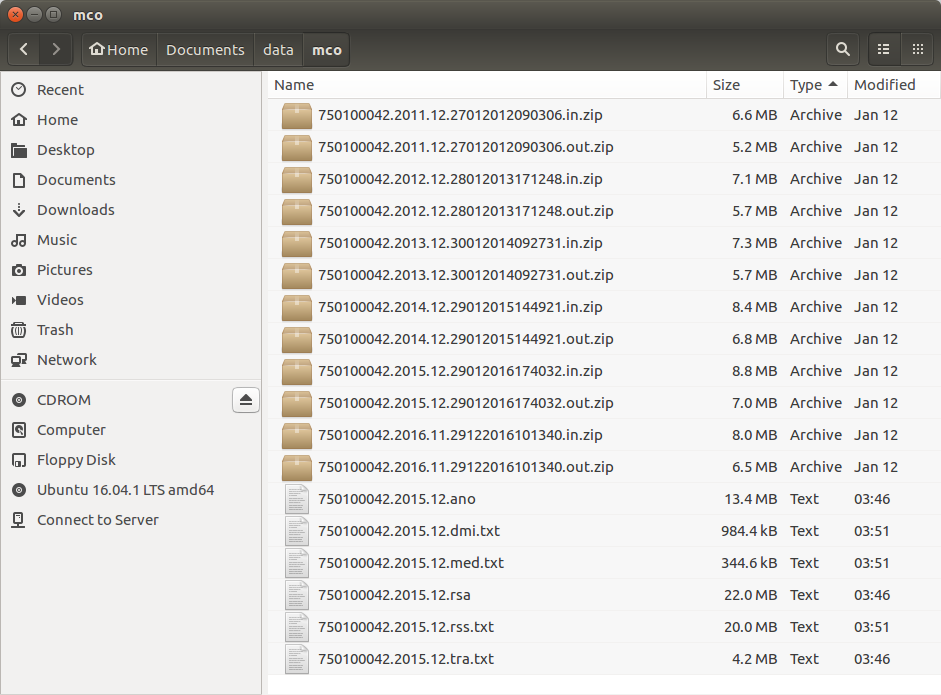
\includegraphics{images/archives_mco_in.png}
\caption{Après éxécution de \texttt{adezip()} sur des fichiers du
\emph{in}}
\end{figure}

\subsection{adelete : effacer}\label{adelete-effacer}

À la fin d'une étude, il est inutile de garder les fichiers dézippés
hors de l'archives, on peut les effacern c'est ce que permet la fonction
\texttt{adelete()}.

\begin{Shaded}
\begin{Highlighting}[]
\CommentTok{# Effacer les fichiers}
\NormalTok{pmeasyr::}\KeywordTok{adelete}\NormalTok{(}\DataTypeTok{finess =} \DecValTok{750100042}\NormalTok{, }
                 \DataTypeTok{annee =} \DecValTok{2015}\NormalTok{, }
                 \DataTypeTok{mois =} \DecValTok{12}\NormalTok{, }
                 \DataTypeTok{path =} \StringTok{'~/Documents/data/mco'}\NormalTok{, }
                 \DataTypeTok{liste =} \KeywordTok{c}\NormalTok{(}\StringTok{"rsa"}\NormalTok{, }\StringTok{"ano"}\NormalTok{, }\StringTok{"tra"}\NormalTok{), }
                 \DataTypeTok{type =} \StringTok{"out"}\NormalTok{)}

\NormalTok{pmeasyr::}\KeywordTok{adelete}\NormalTok{(}\DataTypeTok{finess =} \DecValTok{750100042}\NormalTok{, }
                 \DataTypeTok{annee =} \DecValTok{2015}\NormalTok{, }
                 \DataTypeTok{mois =} \DecValTok{12}\NormalTok{, }
                 \DataTypeTok{path =} \StringTok{'~/Documents/data/mco'}\NormalTok{, }
                 \DataTypeTok{liste =} \KeywordTok{c}\NormalTok{(}\StringTok{"rss"}\NormalTok{, }\StringTok{"med"}\NormalTok{, }\StringTok{"dmi"}\NormalTok{), }
                 \DataTypeTok{type =} \StringTok{"in"}\NormalTok{)}
\end{Highlighting}
\end{Shaded}

\begin{figure}[htbp]
\centering
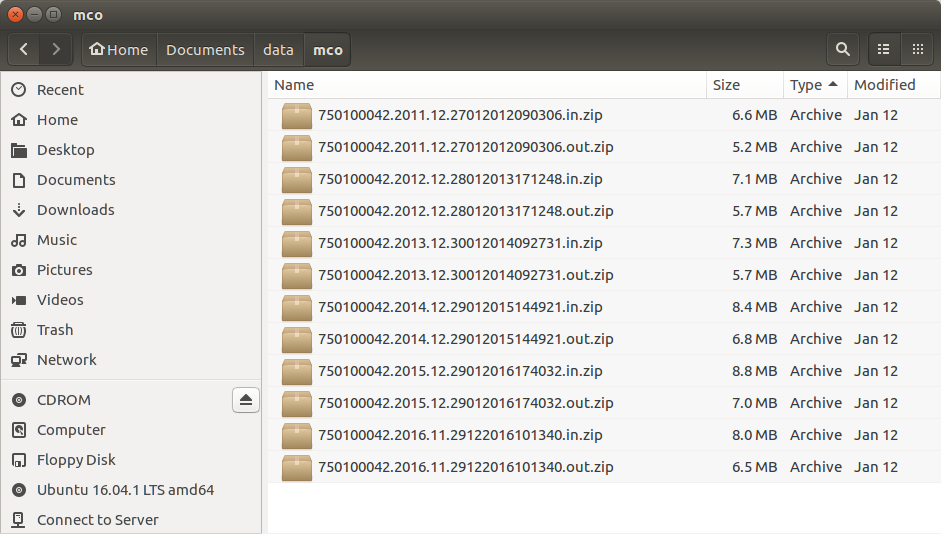
\includegraphics{images/archives_mco.png}
\caption{Après éxécution de \texttt{adelete()}}
\end{figure}

\chapter{Import des données}\label{import-des-donnees}

\section{MCO}\label{mco}

\begin{longtable}[]{@{}ll@{}}
\toprule
Nom & Fonction\tabularnewline
\midrule
\endhead
\href{https://github.com/IM-APHP/pmeasyr/tree/master/Rd_md/irsa.Rmd}{irsa}
& \textasciitilde{} MCO - Import des RSA\tabularnewline
\href{https://github.com/IM-APHP/pmeasyr/tree/master/Rd_md/irum.Rmd}{irum}
& \textasciitilde{} MCO - Import des RUM\tabularnewline
\href{https://github.com/IM-APHP/pmeasyr/tree/master/Rd_md/idiap.Rmd}{idiap}
& \textasciitilde{} MCO - Import des DIAP\tabularnewline
\href{https://github.com/IM-APHP/pmeasyr/tree/master/Rd_md/idmi_mco.Rmd}{idmi\_mco}
& \textasciitilde{} MCO - Import des DMI\tabularnewline
\href{https://github.com/IM-APHP/pmeasyr/tree/master/Rd_md/iium.Rmd}{iium}
& \textasciitilde{} MCO - Import des donnees UM\tabularnewline
\href{https://github.com/IM-APHP/pmeasyr/tree/master/Rd_md/ileg_mco.Rmd}{ileg\_mco}
& \textasciitilde{} MCO - Import des erreurs Leg\tabularnewline
\href{https://github.com/IM-APHP/pmeasyr/tree/master/Rd_md/imed_mco.Rmd}{imed\_mco}
& \textasciitilde{} MCO - Import des Med\tabularnewline
\href{https://github.com/IM-APHP/pmeasyr/tree/master/Rd_md/ipo.Rmd}{ipo}
& \textasciitilde{} MCO - Import des PO\tabularnewline
\href{https://github.com/IM-APHP/pmeasyr/tree/master/Rd_md/iano_mco.Rmd}{iano\_mco}
& \textasciitilde{} MCO - Import des Anohosp\tabularnewline
\bottomrule
\end{longtable}

Les donnees in / out sont prises en charge.

\subsection{RSA}\label{rsa}

Selon la nature des analyses a produire, plusieurs types d'imports sont
possibles :

\begin{longtable}[]{@{}rl@{}}
\toprule
\begin{minipage}[b]{0.06\columnwidth}\raggedleft\strut
Type\strut
\end{minipage} & \begin{minipage}[b]{0.88\columnwidth}\raggedright\strut
Import\strut
\end{minipage}\tabularnewline
\midrule
\endhead
\begin{minipage}[t]{0.06\columnwidth}\raggedleft\strut
1\strut
\end{minipage} & \begin{minipage}[t]{0.88\columnwidth}\raggedright\strut
Light : Partie fixe\strut
\end{minipage}\tabularnewline
\begin{minipage}[t]{0.06\columnwidth}\raggedleft\strut
2\strut
\end{minipage} & \begin{minipage}[t]{0.88\columnwidth}\raggedright\strut
Light+ : Partie fixe + stream en ligne (+) actes et das\strut
\end{minipage}\tabularnewline
\begin{minipage}[t]{0.06\columnwidth}\raggedleft\strut
3\strut
\end{minipage} & \begin{minipage}[t]{0.88\columnwidth}\raggedright\strut
Light++ : Partie fixe + stream en ligne (++) actes, das, typaut um et
dpdr des um\strut
\end{minipage}\tabularnewline
\begin{minipage}[t]{0.06\columnwidth}\raggedleft\strut
4\strut
\end{minipage} & \begin{minipage}[t]{0.88\columnwidth}\raggedright\strut
Standard : Partie fixe + creation des tables actes, das et rsa\_um\strut
\end{minipage}\tabularnewline
\begin{minipage}[t]{0.06\columnwidth}\raggedleft\strut
5\strut
\end{minipage} & \begin{minipage}[t]{0.88\columnwidth}\raggedright\strut
Standard+ : Partie fixe + creation des tables actes, das et rsa\_um +
stream (+)\strut
\end{minipage}\tabularnewline
\begin{minipage}[t]{0.06\columnwidth}\raggedleft\strut
6\strut
\end{minipage} & \begin{minipage}[t]{0.88\columnwidth}\raggedright\strut
Standard++ : Partie fixe + creation des tables actes, das et rsa\_um +
stream (++)\strut
\end{minipage}\tabularnewline
\bottomrule
\end{longtable}

\begin{Shaded}
\begin{Highlighting}[]
\KeywordTok{library}\NormalTok{(pmeasyr)}
\CommentTok{# Import des rsa 2015 type 6}
\KeywordTok{irsa}\NormalTok{(}\DataTypeTok{finess =} \DecValTok{750100042}\NormalTok{, }
     \DataTypeTok{annee =} \DecValTok{2015}\NormalTok{, }
     \DataTypeTok{mois =} \DecValTok{12}\NormalTok{, }
     \DataTypeTok{path =} \StringTok{'~/Documents/data/mco'}\NormalTok{, }
     \DataTypeTok{typi =} \DecValTok{6}\NormalTok{) ->}\StringTok{ }\NormalTok{rsa15}
\KeywordTok{View}\NormalTok{(rsa15$rsa)}
\KeywordTok{View}\NormalTok{(rsa15$rsa_um)}
\KeywordTok{View}\NormalTok{(rsa15$actes)}
\KeywordTok{View}\NormalTok{(rsa15$das)}
\end{Highlighting}
\end{Shaded}

Les tables sont par défaut avec des libellés :

\begin{figure}[htbp]
\centering
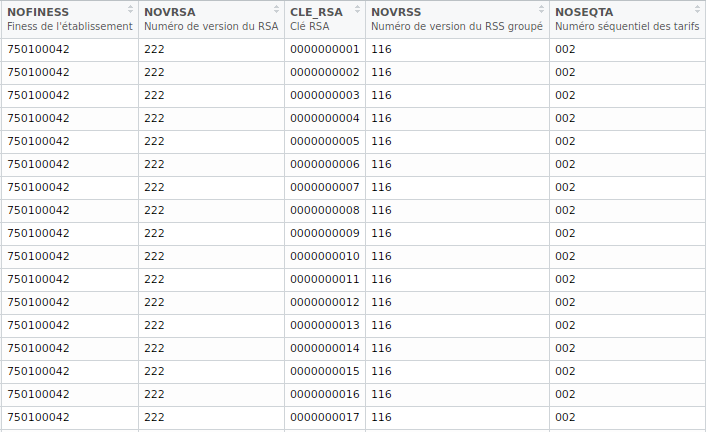
\includegraphics{images/rsa1.png}
\caption{Capture d'une portion de la table \texttt{rsa15\$rsa}}
\end{figure}

\subsection{RUM}\label{rum}

\begin{Shaded}
\begin{Highlighting}[]
\CommentTok{# Import des rsum 2015}
\KeywordTok{irum}\NormalTok{(}\DataTypeTok{finess =} \DecValTok{750100042}\NormalTok{, }
     \DataTypeTok{annee =} \DecValTok{2015}\NormalTok{, }
     \DataTypeTok{mois =} \DecValTok{12}\NormalTok{, }
     \DataTypeTok{path =} \StringTok{'~/Documents/data/mco'}\NormalTok{)}
\end{Highlighting}
\end{Shaded}

Selon la nature des analyses a produire, plusieurs types d'imports sont
possibles :

\begin{longtable}[]{@{}rl@{}}
\toprule
Type & Import\tabularnewline
\midrule
\endhead
1 & XLight : Partie fixe\tabularnewline
2 & Light : Partie fixe + stream en ligne des actes, das et
dad\tabularnewline
3 & Standard : Partie fixe + table actes, das, dad\tabularnewline
4 & Standard+ : Partie fixe + stream + table actes, das,
dad\tabularnewline
\bottomrule
\end{longtable}

\subsection{Colonnes stream}\label{colonnes-stream}

\textbf{Exemples sur quelques rsa} :

\begin{itemize}
\tightlist
\item
  actes : Actes CCAM du Rsa
\end{itemize}

\begin{longtable}[]{@{}rl@{}}
\toprule
Cle RSA & actes\tabularnewline
\midrule
\endhead
0000000001 & EDSF004, EDSF004, JQGA004, JQGA004\tabularnewline
0000000002 & EPLF002, DEQP003, DEQP007, DZQM006\tabularnewline
0000000003 & EBQH002, EEQH002, YYYY180\tabularnewline
\bottomrule
\end{longtable}

\begin{itemize}
\tightlist
\item
  dpdrum : zones diagnostics des passages UM du Rsa
\end{itemize}

\begin{longtable}[]{@{}rl@{}}
\toprule
Cle RSA & dpdrum\tabularnewline
\midrule
\endhead
0000000004 & Z098 I671\tabularnewline
0000000005 & Z380, P741, Z380\tabularnewline
\bottomrule
\end{longtable}

\begin{itemize}
\tightlist
\item
  das : zones diagnostics associes du Rsa
\end{itemize}

\begin{longtable}[]{@{}rl@{}}
\toprule
Cle RSA & das\tabularnewline
\midrule
\endhead
0000000006 & Z9580, Z9588\tabularnewline
0000000007 & P011, P032, P036, P011, P032, P700, P011, P032,
P036\tabularnewline
\bottomrule
\end{longtable}

\begin{itemize}
\tightlist
\item
  um : types autorisations T2A des um de passage par ordre chronologique
\end{itemize}

\begin{longtable}[]{@{}rl@{}}
\toprule
Cle RSA & um\tabularnewline
\midrule
\endhead
0000000009 & 01AC, 53 C\tabularnewline
0000000010 & 51 C\tabularnewline
0000000011 & 71 C, 04 C, 71 C\tabularnewline
\bottomrule
\end{longtable}

\begin{figure}[htbp]
\centering
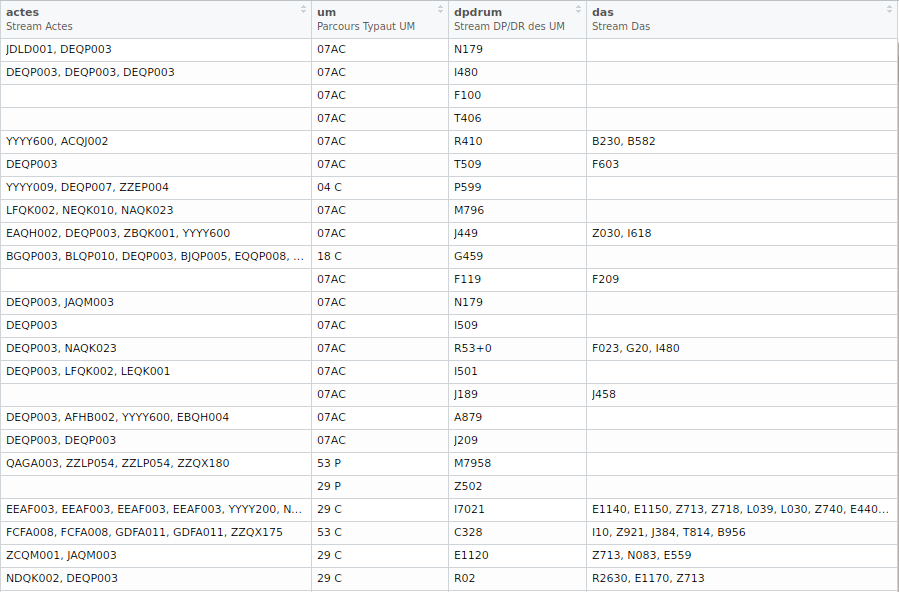
\includegraphics{images/rsa_stream.png}
\caption{Capture des zones \emph{stream} de la table
\texttt{rsa15\$rsa}}
\end{figure}

Pour les quatre autres champs PMSI, seules les donnees du \emph{out}
sont prises en charge par le package pour le moment.

Les fonctions d'imports pour ces trois champs reposent sur le meme
principe qu'en MCO.

\section{HAD}\label{had}

\begin{longtable}[]{@{}ll@{}}
\toprule
Nom & Fonction\tabularnewline
\midrule
\endhead
\href{https://github.com/IM-APHP/pmeasyr/tree/master/Rd_md/iano_had.Rmd}{iano\_had}
& \textasciitilde{} HAD - Import des Anohosp\tabularnewline
\href{https://github.com/IM-APHP/pmeasyr/tree/master/Rd_md/imed_had.Rmd}{imed\_had}
& \textasciitilde{} HAD - Import des Med\tabularnewline
\href{https://github.com/IM-APHP/pmeasyr/tree/master/Rd_md/irapss.Rmd}{irapss}
& \textasciitilde{} HAD - Import des RAPSS\tabularnewline
\bottomrule
\end{longtable}

\begin{Shaded}
\begin{Highlighting}[]
\KeywordTok{irapss}\NormalTok{(}\DataTypeTok{finess =} \DecValTok{750712184}\NormalTok{,}
       \DataTypeTok{annee =} \DecValTok{2015}\NormalTok{,}
       \DataTypeTok{mois =} \DecValTok{12}\NormalTok{,}
       \DataTypeTok{path =} \StringTok{'~/Documents/data/had'}\NormalTok{)}
\end{Highlighting}
\end{Shaded}

\section{SSR}\label{ssr}

\begin{longtable}[]{@{}ll@{}}
\toprule
Nom & Fonction\tabularnewline
\midrule
\endhead
\href{https://github.com/IM-APHP/pmeasyr/tree/master/Rd_md/iano_ssr.Rmd}{iano\_ssr}
& \textasciitilde{} SSR - Import des Anohosp\tabularnewline
\href{https://github.com/IM-APHP/pmeasyr/tree/master/Rd_md/irha.Rmd}{irha}
& \textasciitilde{} SSR - Import des RHA\tabularnewline
\href{https://github.com/IM-APHP/pmeasyr/tree/master/Rd_md/issrha.Rmd}{issrha}
& \textasciitilde{} SSR - Import des SSRHA\tabularnewline
\bottomrule
\end{longtable}

\begin{Shaded}
\begin{Highlighting}[]
\KeywordTok{irha}\NormalTok{(}\DataTypeTok{finess =} \DecValTok{750712184}\NormalTok{,}
       \DataTypeTok{annee =} \DecValTok{2015}\NormalTok{,}
       \DataTypeTok{mois =} \DecValTok{12}\NormalTok{,}
       \DataTypeTok{path =} \StringTok{'~/Documents/data/ssr'}\NormalTok{)}
\end{Highlighting}
\end{Shaded}

\section{PSY}\label{psy}

\begin{longtable}[]{@{}ll@{}}
\toprule
Nom & Fonction\tabularnewline
\midrule
\endhead
\href{https://github.com/IM-APHP/pmeasyr/tree/master/Rd_md/iano_psy.Rmd}{iano\_psy}
& \textasciitilde{} PSY - Import des Anohosp\tabularnewline
\href{https://github.com/IM-APHP/pmeasyr/tree/master/Rd_md/ir3a.Rmd}{ir3a}
& \textasciitilde{} PSY - Import des R3A\tabularnewline
\href{https://github.com/IM-APHP/pmeasyr/tree/master/Rd_md/irpsa.Rmd}{irpsa}
& \textasciitilde{} PSY - Import des RPSA\tabularnewline
\bottomrule
\end{longtable}

\begin{Shaded}
\begin{Highlighting}[]
\KeywordTok{irpsa}\NormalTok{(}\DataTypeTok{finess =} \DecValTok{750712184}\NormalTok{,}
       \DataTypeTok{annee =} \DecValTok{2015}\NormalTok{,}
       \DataTypeTok{mois =} \DecValTok{12}\NormalTok{,}
       \DataTypeTok{path =} \StringTok{'~/Documents/data/psy'}\NormalTok{)}
\end{Highlighting}
\end{Shaded}

\section{RSF}\label{rsf}

\begin{longtable}[]{@{}ll@{}}
\toprule
Nom & Fonction\tabularnewline
\midrule
\endhead
\href{https://github.com/IM-APHP/pmeasyr/tree/master/Rd_md/irafael.Rmd}{irafael}
& \textasciitilde{} RSF - Import des RSFA / Rafael\tabularnewline
\href{https://github.com/IM-APHP/pmeasyr/tree/master/Rd_md/iano_rafael.Rmd}{iano\_rafael}
& \textasciitilde{} RSF - Import des RSFA / ANO\tabularnewline
\bottomrule
\end{longtable}

\begin{Shaded}
\begin{Highlighting}[]
\KeywordTok{irafael}\NormalTok{(}\DataTypeTok{finess =} \DecValTok{750712184}\NormalTok{,}
        \DataTypeTok{annee =} \DecValTok{2015}\NormalTok{,}
        \DataTypeTok{mois =} \DecValTok{12}\NormalTok{,}
        \DataTypeTok{path =} \StringTok{'~/Documents/data/rsf'}\NormalTok{)}
\end{Highlighting}
\end{Shaded}

\chapter{Requêtes sur des pathologies /
actes}\label{requetes-sur-des-pathologies-actes}

\section{Exemple 1 : recherche de codes diagnostics
d'épilepsie}\label{exemple-1-recherche-de-codes-diagnostics-depilepsie}

L'objectif est de récupérer les séjours présentant un code diagnostic de
la liste

\begin{Shaded}
\begin{Highlighting}[]
\CommentTok{# Liste D-0103 de la fonction groupage 2016 : Epilepsies}
\NormalTok{liste_diag =}\StringTok{ }\KeywordTok{c}\NormalTok{(}\StringTok{'F803'}\NormalTok{, }\StringTok{'G400'}\NormalTok{, }\StringTok{'G401'}\NormalTok{, }\StringTok{'G402'}\NormalTok{, }\StringTok{'G403'}\NormalTok{, }\StringTok{'G404'}\NormalTok{, }
               \StringTok{'G405'}\NormalTok{, }\StringTok{'G406'}\NormalTok{, }\StringTok{'G407'}\NormalTok{, }\StringTok{'G408'}\NormalTok{, }\StringTok{'G409'}\NormalTok{, }\StringTok{'G410'}\NormalTok{, }
               \StringTok{'G411'}\NormalTok{, }\StringTok{'G412'}\NormalTok{, }\StringTok{'G418'}\NormalTok{, }\StringTok{'G419'}\NormalTok{, }\StringTok{'R568'}\NormalTok{)}

\NormalTok{## En passant par la table diags}
\KeywordTok{tdiag}\NormalTok{(rsa15) ->}\StringTok{ }\NormalTok{rsa15}

\KeywordTok{library}\NormalTok{(dplyr)}
\CommentTok{# quel que soit la position du diagnostic}
\NormalTok{rsa15$diags %>%}\StringTok{ }\KeywordTok{filter}\NormalTok{(diag %in%}\StringTok{ }\NormalTok{liste_diag)}
\CommentTok{# position en das}
\NormalTok{rsa15$diags %>%}\StringTok{ }\KeywordTok{filter}\NormalTok{(diag %in%}\StringTok{ }\NormalTok{liste_diag, position ==}\StringTok{ }\DecValTok{5}\NormalTok{)}
\CommentTok{# position en dp dr}
\NormalTok{rsa15$diags %>%}\StringTok{ }\KeywordTok{filter}\NormalTok{(diag %in%}\StringTok{ }\NormalTok{liste_diag, position <}\StringTok{ }\DecValTok{5}\NormalTok{)}

\NormalTok{## En passant par les zones stream}
\NormalTok{string_diags =}\StringTok{ }
\StringTok{  'F803|G400|G401|G402|G403|G404|G405|G406|G407|G408|G409|G410|G411|G412|418|G419|R568'}

\CommentTok{# quel que soit la position du diagnostic}
\NormalTok{rsa15$rsa %>%}\StringTok{ }\KeywordTok{fiter}\NormalTok{(}\KeywordTok{grepl}\NormalTok{(string_diags, dpdrum)|}\KeywordTok{grepl}\NormalTok{(string_diags, das))}
\CommentTok{# position en das}
\NormalTok{rsa15$rsa %>%}\StringTok{ }\KeywordTok{fiter}\NormalTok{(}\KeywordTok{grepl}\NormalTok{(string_diags, das))}
\CommentTok{# position en dpdr}
\NormalTok{rsa15$rsa %>%}\StringTok{ }\KeywordTok{fiter}\NormalTok{(}\KeywordTok{grepl}\NormalTok{(string_diags, dpdrum))}
\end{Highlighting}
\end{Shaded}

\section{Exemple 2 : recherche de codes actes de pose de
PAC}\label{exemple-2-recherche-de-codes-actes-de-pose-de-pac}

\begin{Shaded}
\begin{Highlighting}[]
\CommentTok{# Code EBLA003}

\KeywordTok{library}\NormalTok{(dplyr)}
\CommentTok{# En pssant par la table actes}
\NormalTok{rsa15$actes %>%}\StringTok{ }\KeywordTok{filter}\NormalTok{(CDCCAM ==}\StringTok{ 'EBLA003'}\NormalTok{)}
\CommentTok{# En pssant par la zone stream}
\NormalTok{rsa15$rsa %>%}\StringTok{ }\KeywordTok{filter}\NormalTok{(}\KeywordTok{grepl}\NormalTok{(}\StringTok{'EBLA003'}\NormalTok{, actes))}
\end{Highlighting}
\end{Shaded}

\chapter{étude des files actives}\label{etude-des-files-actives}

We have finished a nice book.

\chapter{Chaînage PMSI}\label{chainage-pmsi}

We have finished a nice book.

\chapter{Statistiques descriptives}\label{statistiques-descriptives}

We describe our methods in this chapter.

\chapter{Visualiser}\label{visualiser}

\section{Visualiser l'activité}\label{visualiser-lactivite}

\section{Visualiser le groupage}\label{visualiser-le-groupage}


\end{document}
